\documentclass[conference]{IEEEtran}
\IEEEoverridecommandlockouts
\usepackage{cite}
\usepackage{amsmath,amssymb,amsfonts}
\usepackage{graphicx}
\usepackage{booktabs}
\usepackage{array}
\usepackage{url}
\usepackage{xcolor}
\usepackage{hyperref}
\hypersetup{colorlinks=true,linkcolor=black,citecolor=black,urlcolor=blue}

\begin{document}

\title{FinRAG: Domain-Adaptive Fine-Tuning of Retrieval, Reranking, and Generation for Financial Report Question Answering}

\author{
\IEEEauthorblockN{Haroon Bilal}
\IEEEauthorblockA{\textit{Department of Computer Science} \\
\textit{Your University}\\
City, Country \\
haroonmbilal007@gmail.com}
\and
\IEEEauthorblockN{Muhammad Sarwar}
\IEEEauthorblockA{\textit{Department of Computer Science} \\
\textit{Your University}\\
City, Country \\
muhammad.b.sarwar8@gmail.com}
}

\maketitle

\begin{abstract}
Question answering over financial reports is hard: the documents are long, the questions are
written in short analyst shorthand, and many answers require small calculations. Most existing
Retrieval-Augmented Generation (RAG) systems for finance use general-purpose, off-the-shelf
models and a paid large language model (LLM), and they are usually evaluated only on the quality
of the final written answer. In this work we build FinRAG, a RAG system that runs completely on a
single laptop GPU (an RTX~4080 with 12~GB of memory) and uses no paid services. We fine-tune all
three main parts of the pipeline on the FinDER benchmark of S\&P~500 annual reports: the embedding
model used for search, the cross-encoder reranker, and a 7B generator trained with QLoRA. We also
report retrieval metrics (MRR, NDCG, Recall) against the gold evidence, which the closest prior
work did not report. On 5{,}625 questions, fine-tuning the embedder raises MRR@10 from 0.087 to
0.260 (about $3\times$) and Recall@10 from 0.159 to 0.404 over the strongest off-the-shelf baseline.
On 300 held-out questions, QLoRA improves generation ROUGE-L from 0.077 to 0.203 and BERTScore-F1
from 0.824 to 0.866. Interestingly, our ablation shows that once the embedder is fine-tuned, adding
sparse fusion or reranking barely helps at the top ranks --- which is different from earlier work that
found reranking useful for generic embedders. Our main takeaway is that, for a specific domain,
fine-tuning the retriever matters most.
\end{abstract}

\begin{IEEEkeywords}
retrieval-augmented generation, dense retrieval, fine-tuning, reranking, financial NLP, question
answering, QLoRA, information retrieval
\end{IEEEkeywords}

\section{Introduction}
Financial analysts spend a lot of time reading annual reports (the U.S. Securities and Exchange
Commission Form 10-K) to answer fairly specific questions, such as how a company's revenue changed
between two years or what risk factors it disclosed. Large language models (LLMs) can help with this,
but they are prone to making up numbers when asked about a specific company. Retrieval-Augmented
Generation (RAG)~\cite{lewis2020rag} reduces this problem by first searching a document collection for
relevant passages and then letting the model write its answer using those passages. This keeps the
answer grounded in a real source.

A typical RAG system has two stages. The first stage \emph{retrieves} candidate passages, often using a
dense embedding model~\cite{karpukhin2020dpr} together with a classic keyword method such as
BM25~\cite{robertson2009bm25}. The second stage \emph{generates} the answer with an LLM. Many systems
also add a \emph{reranker} in between, which is a stronger but slower model that re-scores the top
candidates~\cite{nogueira2019passage}.

In the financial domain specifically, we noticed two common problems. First, most systems use
\emph{off-the-shelf} models that were never adapted to finance. Financial questions are short and full
of abbreviations (for example, ``Delta in CBOE Data \& Access Solutions rev from 2021-23''), and the
filings are long and full of numbers, so a generic embedding model often struggles. Second, many papers
only measure how good the final answer is (for example, by asking GPT-4 to grade it) and do not measure
how good the \emph{search} step was, even when the dataset provides the correct evidence passages. This
makes it hard to know whether a wrong answer came from bad search or from bad generation.

This project asks a simple question: if we fine-tune the main RAG components on financial data, using
only a normal gaming laptop and free open-source models, how much better does the system get? Our
contributions are:
\begin{itemize}
\item \textbf{A fully local, free RAG pipeline (FinRAG)} that fine-tunes the embedder, the reranker, and
the generator on FinDER using a single 12~GB GPU and no paid APIs.
\item \textbf{Retrieval metrics that prior work skipped.} We align FinDER's gold evidence to our chunks
and report MRR@10, NDCG@10, and Recall@$\{5,10,20\}$, in addition to standard generation metrics.
\item \textbf{An ablation with a clear finding:} fine-tuning the embedder is by far the biggest
improvement, and once it is done, reranking and sparse fusion add little at the top ranks. We also
report a practical lesson about how reranker negatives must be mined.
\end{itemize}

\section{Related Work}
\textbf{Dense retrieval.} Dense Passage Retrieval (DPR)~\cite{karpukhin2020dpr} showed that two-tower
encoders trained with contrastive learning beat sparse methods such as BM25~\cite{robertson2009bm25} on
open-domain QA. ColBERT~\cite{khattab2020colbert} uses token-level late interaction for higher accuracy
at higher cost. Sentence-BERT~\cite{reimers2019sbert} introduced siamese training for sentence
embeddings. Contriever~\cite{izacard2022contriever}, E5~\cite{wang2022e5}, GTR~\cite{ni2022gtr}, and the
BGE family~\cite{xiao2023bge} are strong general-purpose embedding models; BGE in particular is trained
with hard-negative contrastive learning and is a common RAG retriever, which is why we build on it.
BEIR~\cite{thakur2021beir} is a popular benchmark for comparing such retrievers in a zero-shot setting.

\textbf{Reranking.} Cross-encoder rerankers read the query and a candidate passage together and output a
relevance score~\cite{nogueira2019passage}. They are the standard ``second stage'' that refines the
output of a fast first-stage retriever, and they were the main focus of the financial RAG work we extend.

\textbf{Fusion of dense and sparse retrieval.} Combining a dense retriever with BM25 is a common way to
get the benefits of both. Reciprocal Rank Fusion (RRF)~\cite{cormack2009rrf} is a simple and effective
way to merge two ranked lists, and we use it here. HyDE~\cite{gao2022hyde} is another retrieval trick that
generates a hypothetical document first; we do not use it but mention it for completeness.

\textbf{Retrieval-augmented generation.} Beyond the original RAG model~\cite{lewis2020rag}, Fusion-in-Decoder
\cite{izacard2021fid} and Self-RAG~\cite{asai2023selfrag} explore different ways of using retrieved text
during generation. The Transformer architecture~\cite{vaswani2017attention} underlies all of these models.

\textbf{Parameter-efficient fine-tuning.} Full fine-tuning of a 7B model does not fit on a 12~GB GPU.
LoRA~\cite{hu2021lora} trains only small low-rank update matrices, and QLoRA~\cite{dettmers2023qlora}
adds 4-bit quantization so that a 7B model can be fine-tuned on a single consumer card. We use QLoRA for
our generator. Our generator backbone is Qwen2.5~\cite{qwen2024}; other popular open models include
Llama~\cite{touvron2023llama} and Mistral~\cite{jiang2023mistral}.

\textbf{Financial NLP.} Earlier domain models include FinBERT~\cite{araci2019finbert} and
BloombergGPT~\cite{wu2023bloomberggpt}. FinQA~\cite{chen2021finqa} introduced numerical reasoning over
financial reports, and FinDER~\cite{finder2025} is the retrieval-focused benchmark we use, built on
S\&P~500 10-K filings with gold evidence.

\textbf{RAG evaluation.} RAGAS~\cite{es2023ragas} measures faithfulness and answer relevance. For
generation we use ROUGE~\cite{lin2004rouge}, BLEU~\cite{papineni2002bleu}, and
BERTScore~\cite{zhang2020bertscore}; for retrieval we use standard metrics summarized in IR
textbooks~\cite{manning2008ir}, and FAISS~\cite{johnson2019faiss} for the vector index.

\textbf{Base reference.} We build directly on Cheng~\textit{et al.}~\cite{basepaper2026}, who built a
financial RAG system on FinDER using hybrid retrieval and a cross-encoder reranker, but with
\emph{off-the-shelf} embeddings and a \emph{paid} LLM (for both query rewriting and answer generation),
and who evaluated only with an LLM judge. We extend their work by fine-tuning all three components,
running everything locally and for free, and reporting retrieval-side metrics.

\section{Dataset}
We use FinDER~\cite{finder2025}, a financial QA benchmark built on the 10-K annual reports of S\&P~500
companies. After downloading, the version we use contains 497 filings (as HTML) and 5{,}703 questions.
Every question comes with (i) the question text, (ii) a gold answer, and (iii) one or more
\emph{reference} passages --- the actual text from the filing that supports the answer. The reference
passages are what let us measure retrieval quality.

FinDER is deliberately difficult. The questions are short and use heavy abbreviation, the relevant
information is buried inside very long documents, and roughly 15\% of the questions need a small
calculation (subtraction, division, and so on). Table~\ref{tab:dataset} summarizes the dataset as we use
it.

\begin{table}[t]
\caption{FinDER dataset as used in this work.}
\label{tab:dataset}
\centering
\small
\begin{tabular}{ll}
\toprule
Property & Value \\
\midrule
Documents (10-K filings) & 497 \\
Questions & 5{,}703 \\
Chunks after splitting & 155{,}045 \\
Questions aligned to a gold chunk & 5{,}625 (98.6\%) \\
References per question (avg) & 1.07 \\
Question categories & 8 \\
\bottomrule
\end{tabular}
\end{table}

\section{Methodology}
Fig.~\ref{fig:pipeline} shows the full pipeline. We describe each part below.

\begin{figure}[t]
\centering
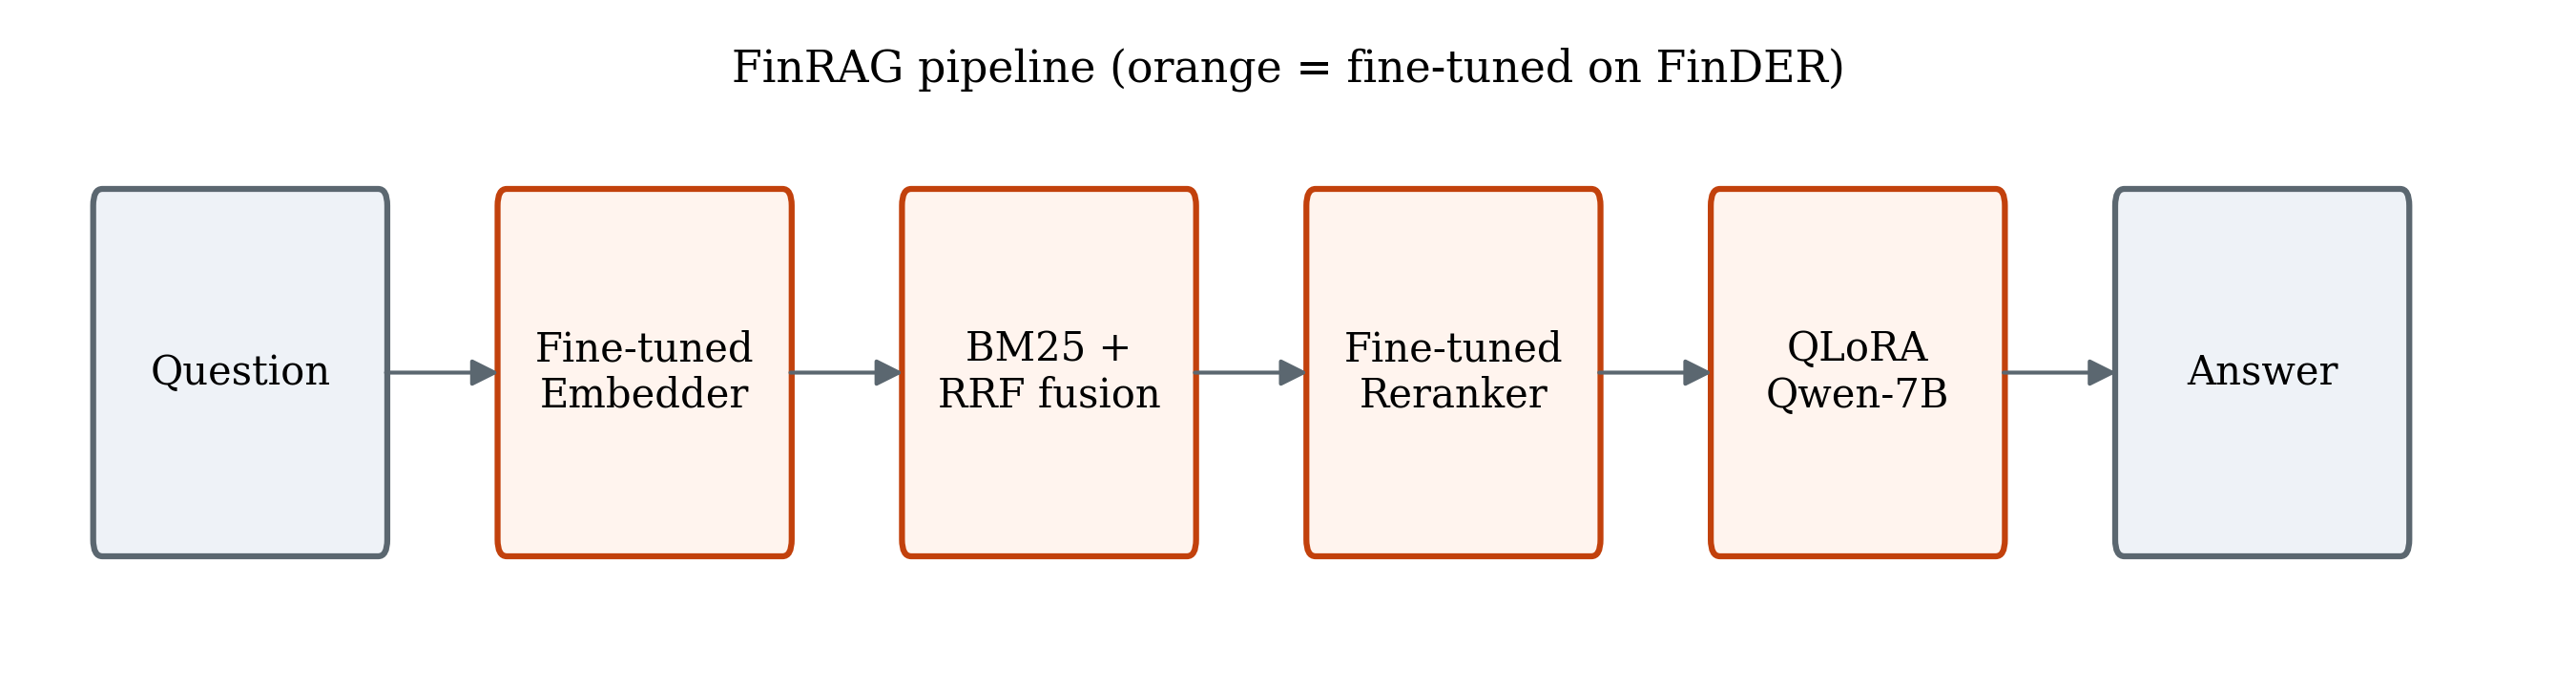
\includegraphics[width=\columnwidth]{fig5_pipeline.png}
\caption{The FinRAG pipeline. The orange boxes are the three components we fine-tuned on FinDER.}
\label{fig:pipeline}
\end{figure}

\subsection{Corpus Construction and Evidence Alignment}
We parse each 10-K HTML file to plain text and split it into overlapping chunks of about 300 words with a
60-word overlap, giving 155{,}045 chunks. FinDER gives the gold evidence as raw text rather than as a
chunk ID, so we have to figure out which of our chunks each gold passage corresponds to. We do this with
TF--IDF: we vectorize all chunks, vectorize each gold reference, and take the chunk with the highest
cosine similarity (above a threshold of 0.30) as the relevant one. This matched 5{,}625 of 5{,}703
questions (98.6\%), and we use these matches as our relevance judgments (qrels).

\subsection{Embedding Fine-Tuning}
The first-stage retriever is \texttt{bge-small-en-v1.5}~\cite{xiao2023bge}. We fine-tune it with the
Multiple Negatives Ranking Loss, which for a batch of queries pulls each query close to its correct
passage and pushes it away from all other passages in the batch (and from explicit hard negatives). With
cosine similarity $s(\cdot,\cdot)$ and temperature $\tau$, the loss for a query $q_i$ with positive
$p_i^{+}$ is
\begin{equation}
\mathcal{L}_i = -\log \frac{\exp\!\big(s(q_i, p_i^{+})/\tau\big)}
{\sum_{j} \exp\!\big(s(q_i, p_j)/\tau\big)},
\end{equation}
where the denominator runs over the positive and all negatives for $q_i$. The hard negatives are mined
with the base model: for each query we retrieve the top passages and keep the highly-ranked ones that are
not the gold chunk, since these are the ``tempting but wrong'' passages the model should learn to avoid.

\subsection{Reranker Fine-Tuning}
The reranker is the cross-encoder \texttt{bge-reranker-base}. We fine-tune it on (query, positive,
negative) pairs, labeling the gold chunk as $1$ and negatives as $0$, with a binary cross-entropy loss.
An important detail we learned the hard way: the negatives must be mined from the \emph{fine-tuned}
retriever, not the base model. The reranker runs behind the fine-tuned retriever at inference time, so
its candidates are all highly relevant and look similar to each other; training it on easy base-model
negatives did not prepare it for this and actually made ranking worse (see Section~\ref{sec:disc}).

\subsection{Generator Fine-Tuning (QLoRA)}
The generator is \texttt{Qwen2.5-7B-Instruct}~\cite{qwen2024}, fine-tuned with QLoRA~\cite{dettmers2023qlora}:
the base weights are loaded in 4-bit (NF4) and frozen, and we train LoRA~\cite{hu2021lora} adapters
(rank 16) on the attention and MLP projection layers. Each training example is a question plus its gold
context, and the target is the gold answer. We mask the prompt tokens so the loss is computed only on the
answer, which teaches the model to \emph{answer} in FinDER's short, numeric style rather than to copy the
context. Only about 0.53\% of the parameters are trained.

\subsection{Retrieval Stack and Fusion}
At inference, the fine-tuned embedder retrieves the top passages from a FAISS~\cite{johnson2019faiss}
inner-product index. We optionally fuse this with a BM25 list using Reciprocal Rank
Fusion~\cite{cormack2009rrf}: a document $d$ gets the score
\begin{equation}
\text{RRF}(d) = \sum_{r \in \{dense, sparse\}} \frac{1}{k + \text{rank}_r(d)}, \quad k = 60,
\end{equation}
and the merged list is optionally reranked by the cross-encoder before the top passages are sent to the
generator.

\subsection{Evaluation Metrics}
For retrieval we report standard metrics~\cite{manning2008ir}. For a set of queries $Q$,
\begin{equation}
\text{MRR@}K = \frac{1}{|Q|}\sum_{i=1}^{|Q|}\frac{1}{\text{rank}_i}, \quad
\text{Recall@}K = \frac{|\,\text{relevant} \cap \text{top-}K\,|}{|\text{relevant}|},
\end{equation}
where $\text{rank}_i$ is the position of the first relevant chunk (or $\infty$ beyond $K$). NDCG@$K$ is
the discounted cumulative gain $\text{DCG@}K = \sum_{i=1}^{K} \text{rel}_i / \log_2(i+1)$ normalized by
its ideal value. For generation we use ROUGE-L~\cite{lin2004rouge}, BLEU~\cite{papineni2002bleu}, and
BERTScore-F1~\cite{zhang2020bertscore} against the gold answers.

\section{Experimental Setup}
Everything runs on one NVIDIA RTX~4080 Laptop GPU (12~GB) with 32~GB of system RAM, using PyTorch,
the \texttt{sentence-transformers} library, FAISS, and \texttt{rank\_bm25}. No paid or external APIs are
used at any point. Table~\ref{tab:hyper} lists the main training settings. We hold out the last 300
questions for generation evaluation so the generator never sees them during training.

\begin{table}[t]
\caption{Training configuration for each fine-tuned component.}
\label{tab:hyper}
\centering
\small
\begin{tabular}{lcccc}
\toprule
Component & Base model & Epochs & Batch & LR \\
\midrule
Embedder & bge-small-en-v1.5 & 3 & 32 & $2\!\times\!10^{-5}$ \\
Reranker & bge-reranker-base & 3 & 16 & $2\!\times\!10^{-5}$ \\
Generator & Qwen2.5-7B-Instruct & 1 & 8\textsuperscript{*} & $2\!\times\!10^{-4}$ \\
\bottomrule
\end{tabular}
\\[2pt]
\footnotesize{\textsuperscript{*}effective batch via gradient accumulation; QLoRA rank 16.}
\end{table}

\section{Results}
\label{sec:results}

\subsection{Retrieval}
Table~\ref{tab:retrieval} shows retrieval results on 5{,}625 questions. Fine-tuning the embedder gives a
large jump: our best configuration (FT~Dense) reaches 0.260 MRR@10 versus 0.087 for the strongest
off-the-shelf baseline (Hybrid+Rerank), about a $3\times$ improvement, and Recall@10 more than doubles.
Fig.~\ref{fig:main} and Fig.~\ref{fig:recall} show this visually.

\begin{table}[t]
\caption{Retrieval performance on FinDER (5{,}625 questions). FT = fine-tuned. Best in \textbf{bold}.}
\label{tab:retrieval}
\centering
\small
\begin{tabular}{lccccc}
\toprule
System & MRR@10 & NDCG@10 & R@5 & R@10 & R@20 \\
\midrule
Dense (off-the-shelf) & 0.064 & 0.076 & 0.091 & 0.122 & 0.151 \\
Hybrid & 0.056 & 0.070 & 0.083 & 0.121 & 0.164 \\
Hybrid + Rerank & 0.087 & 0.102 & 0.127 & 0.159 & 0.198 \\
\midrule
\textbf{FT Dense (ours)} & \textbf{0.260} & \textbf{0.292} & \textbf{0.342} & \textbf{0.404} & \textbf{0.467} \\
FT Hybrid & 0.193 & 0.231 & 0.284 & 0.362 & 0.433 \\
FT Hybrid + Rerank & 0.189 & 0.223 & 0.267 & 0.346 & 0.436 \\
\bottomrule
\end{tabular}
\end{table}

\begin{figure}[t]
\centering
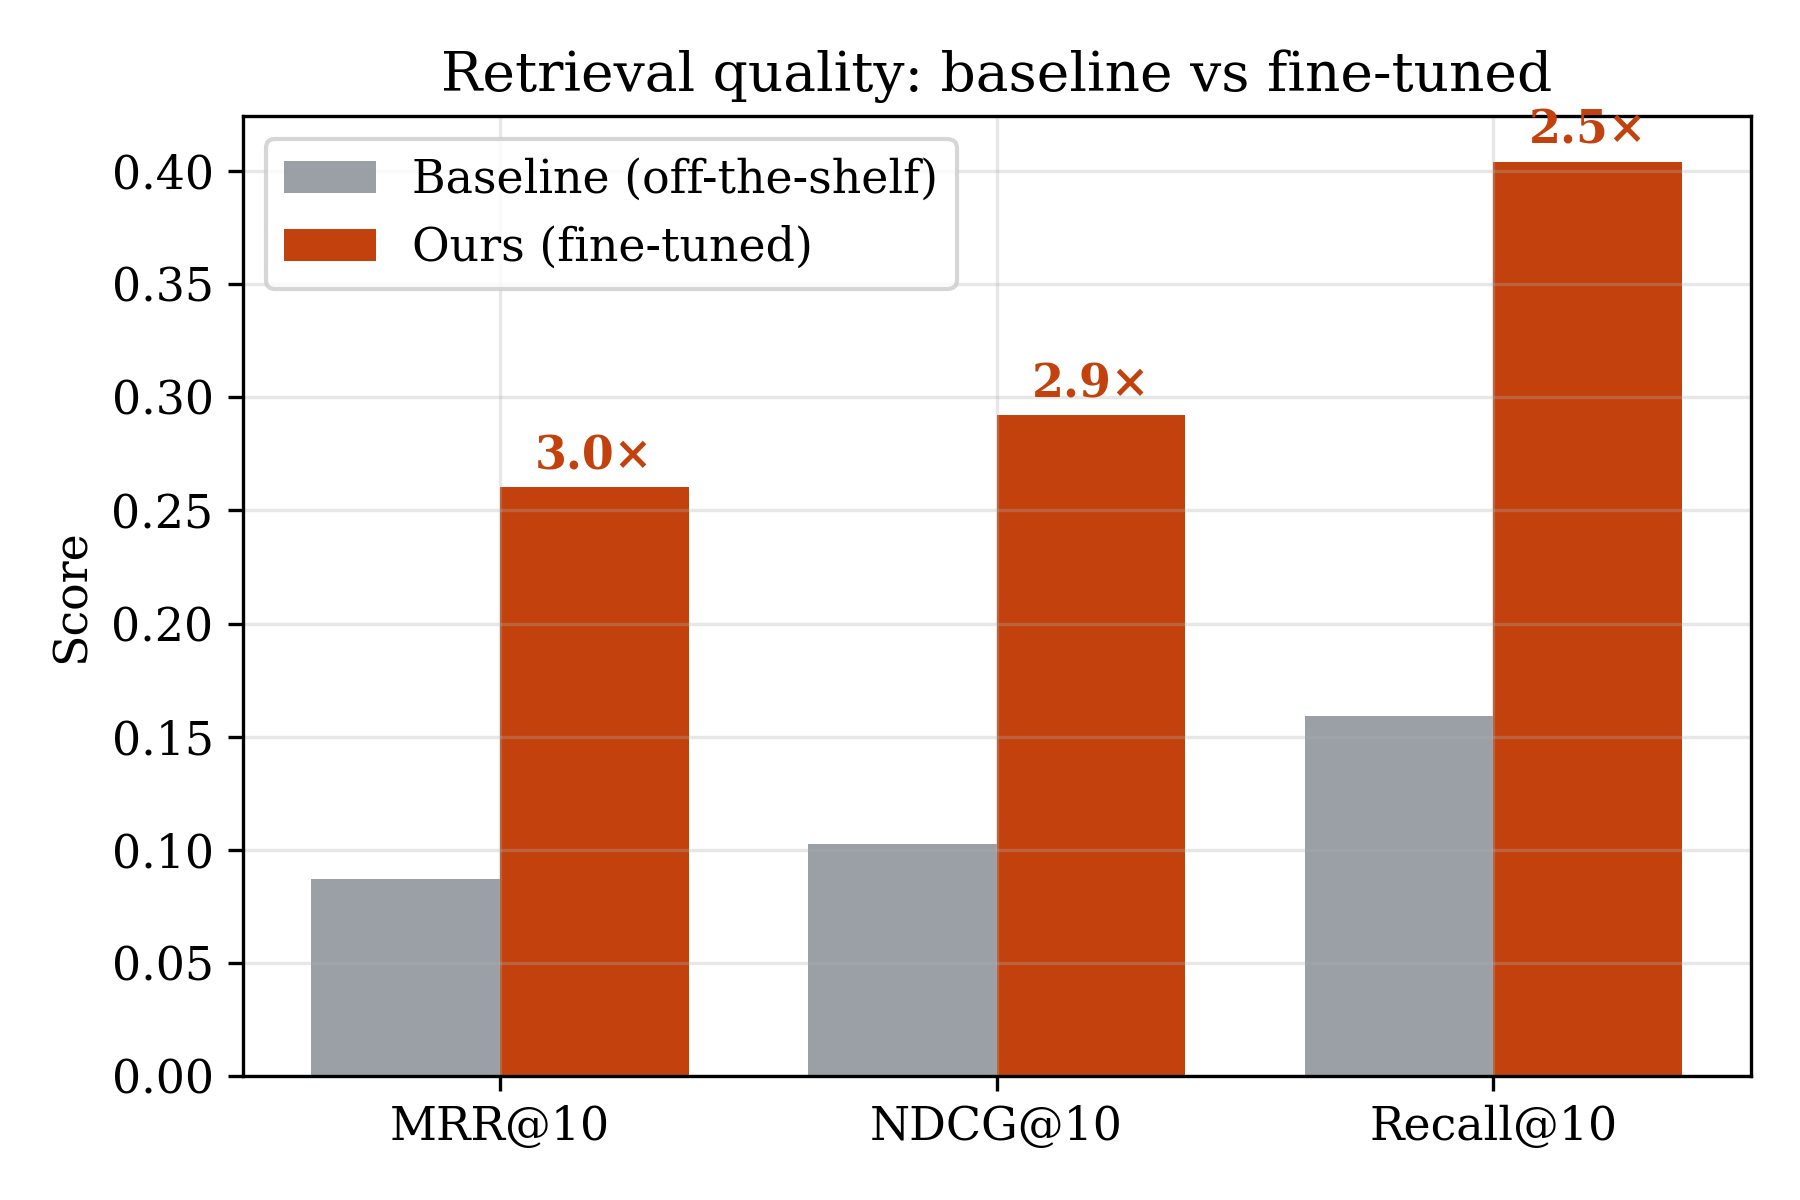
\includegraphics[width=\columnwidth]{fig1_main_comparison.png}
\caption{Retrieval quality: best off-the-shelf baseline versus our fine-tuned system.}
\label{fig:main}
\end{figure}

\begin{figure}[t]
\centering
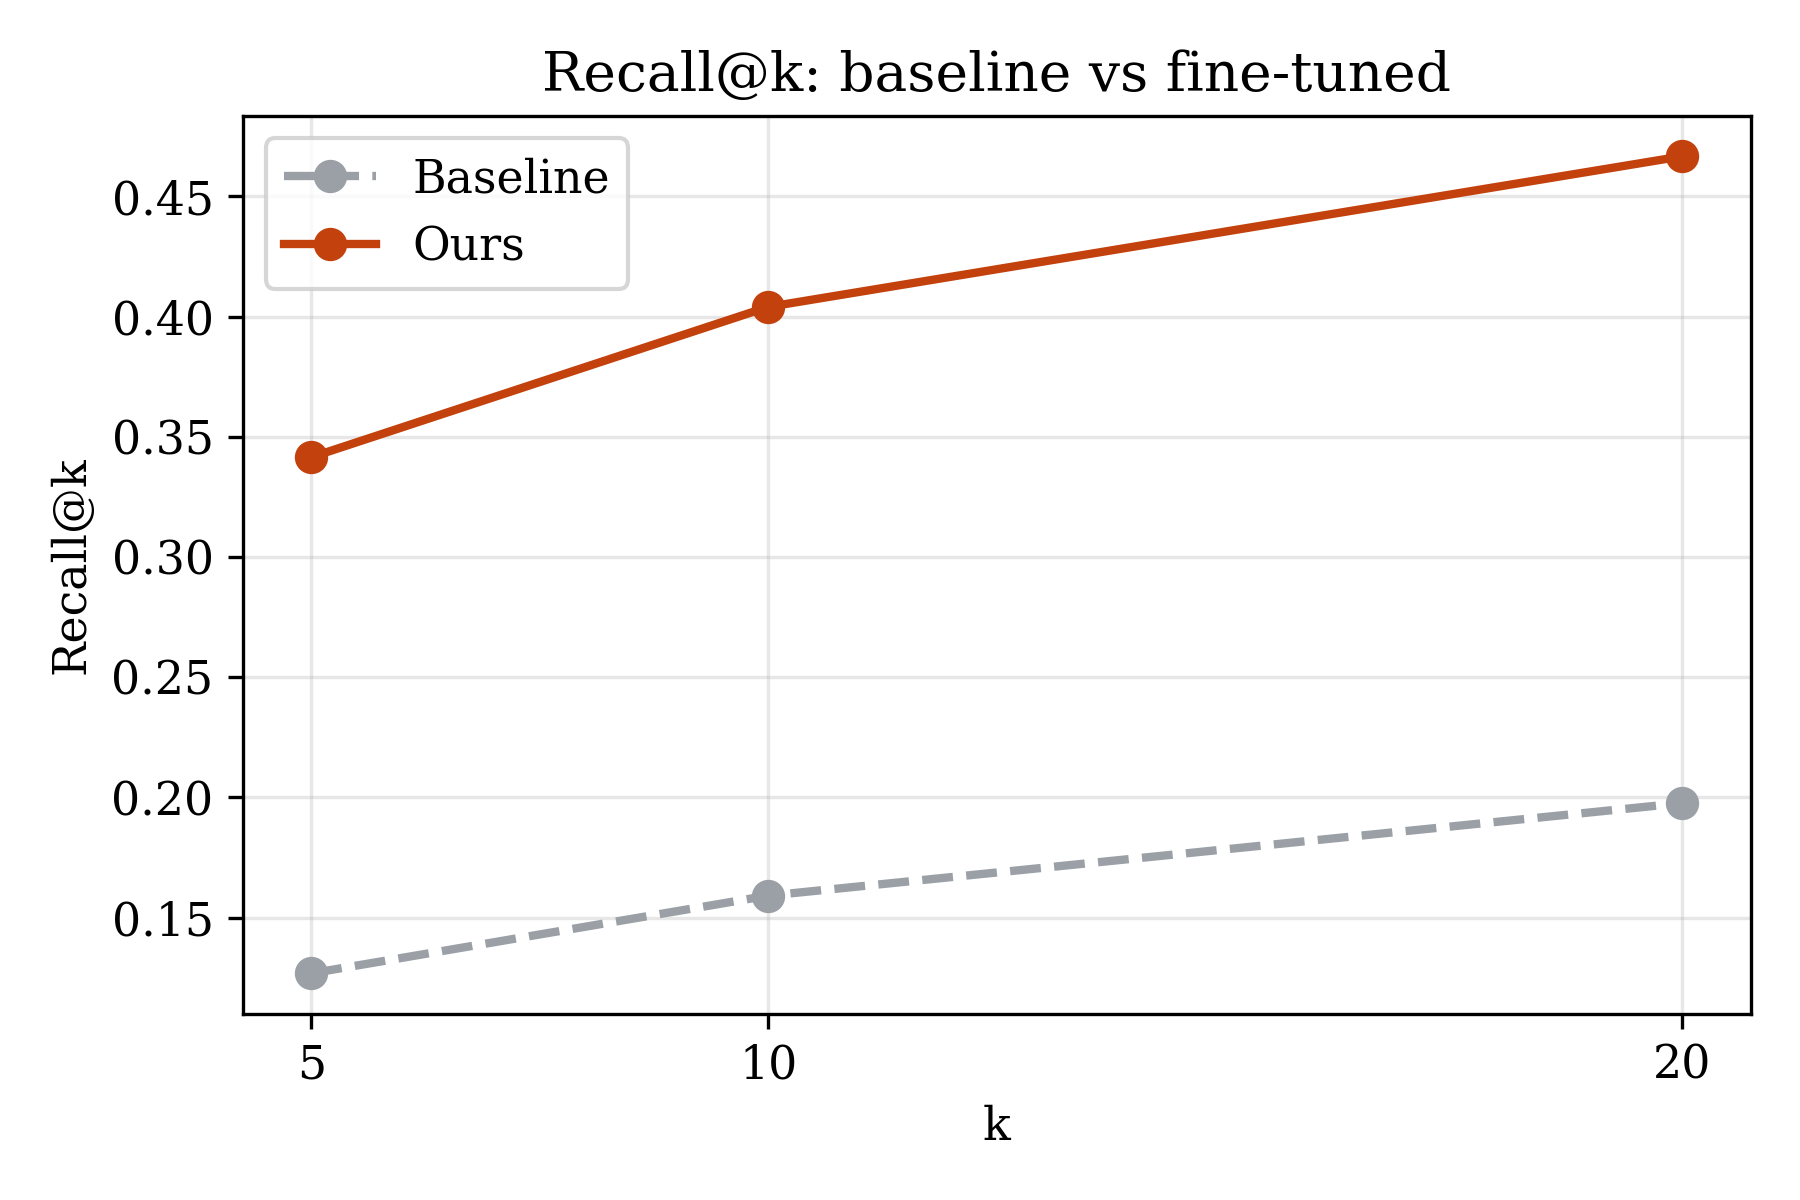
\includegraphics[width=\columnwidth]{fig2_recall_curve.png}
\caption{Recall@$k$ for the baseline and our fine-tuned system.}
\label{fig:recall}
\end{figure}

\subsection{Ablation}
Fig.~\ref{fig:ablation} breaks down the contribution of each component on MRR@10. The fine-tuned dense
retriever alone is the biggest win. Adding BM25 fusion or reranking on top of it does not help at the top
ranks --- in fact FT~Dense beats both FT~Hybrid and FT~Hybrid+Rerank. We discuss why in
Section~\ref{sec:disc}.

\begin{figure}[t]
\centering
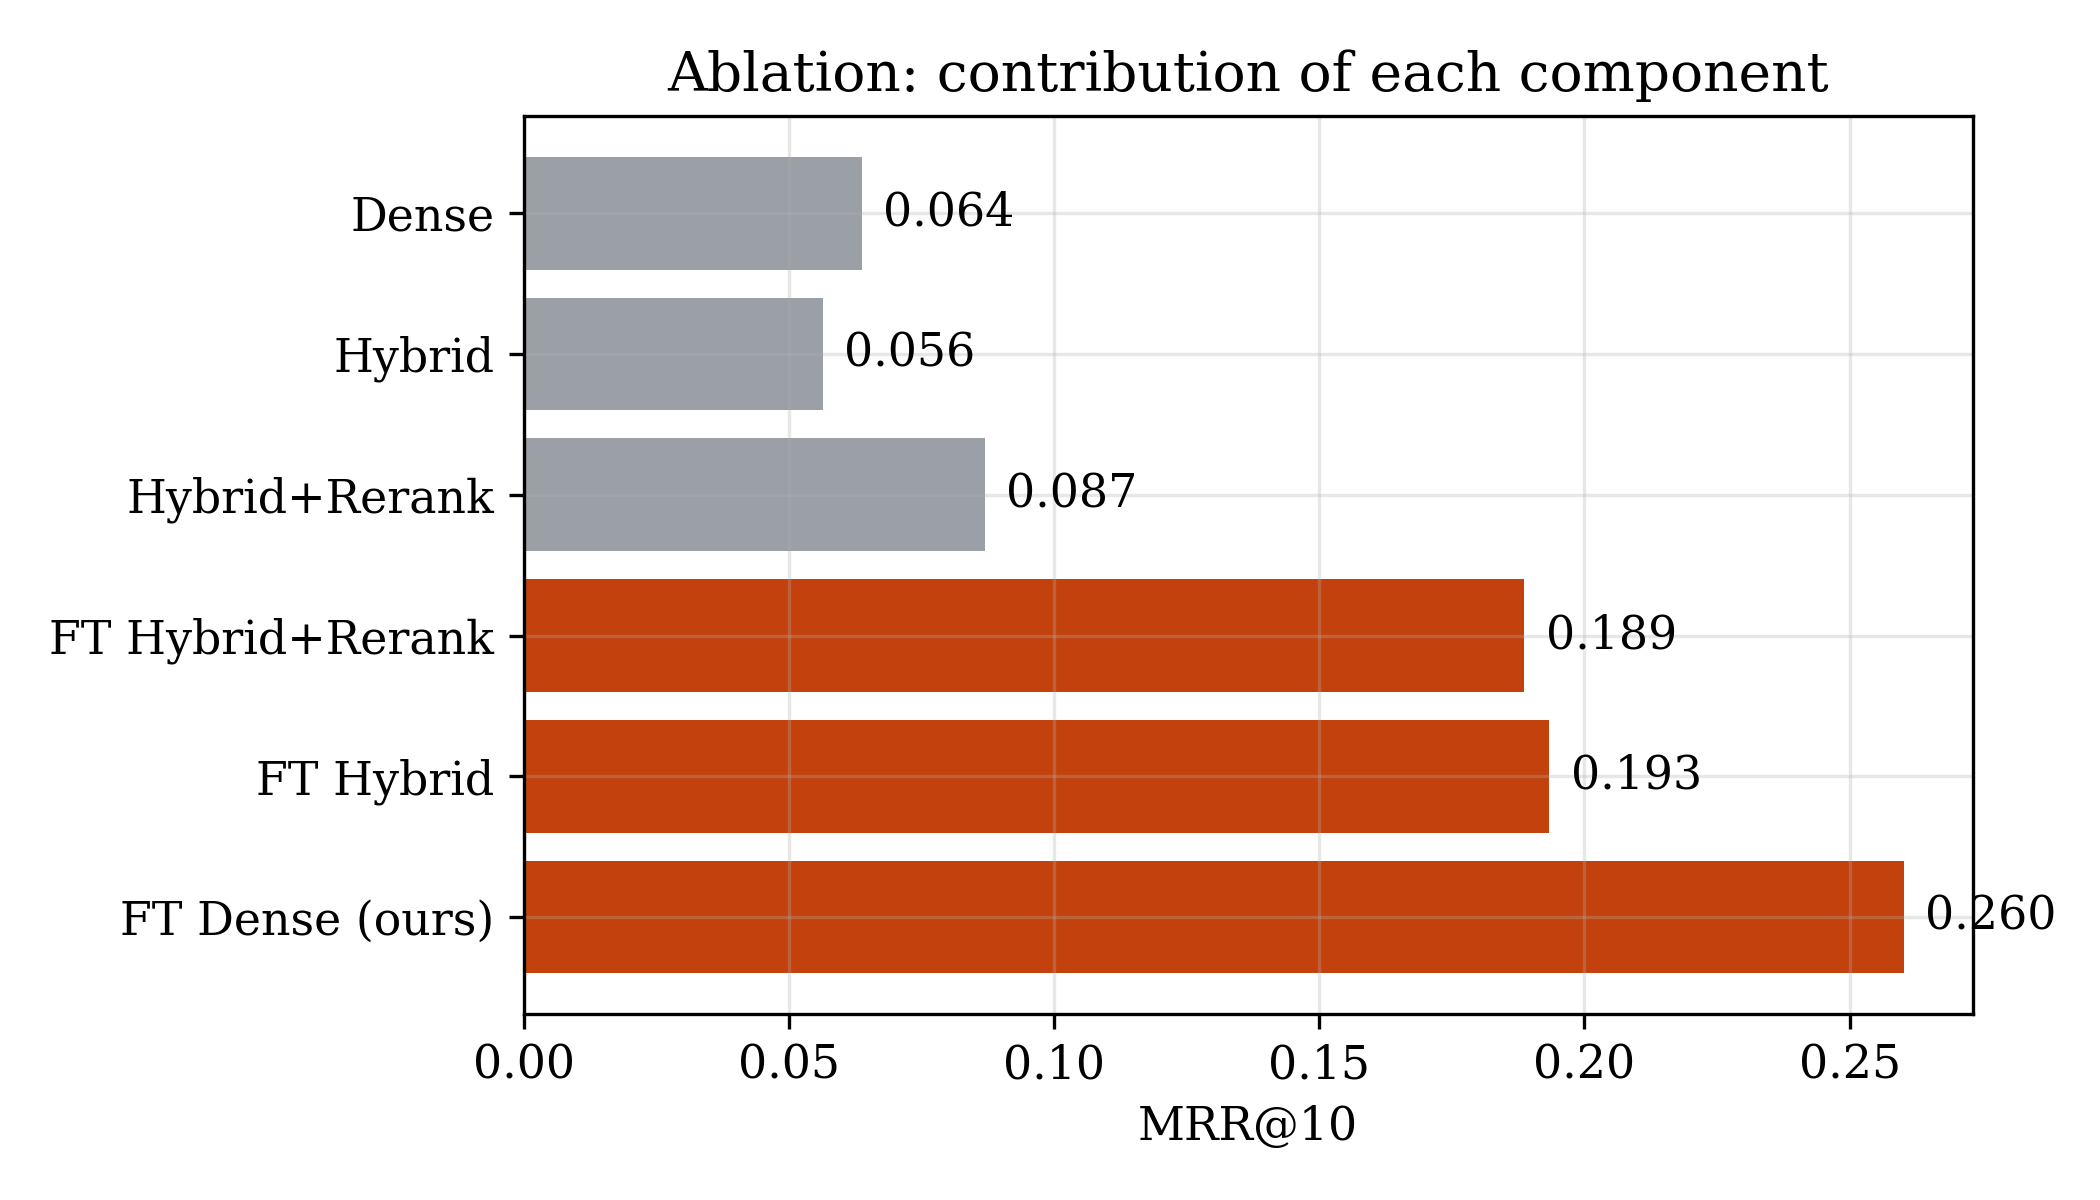
\includegraphics[width=\columnwidth]{fig3_ablation.png}
\caption{Ablation on MRR@10. Grey bars are off-the-shelf; orange bars are fine-tuned.}
\label{fig:ablation}
\end{figure}

\subsection{Generation}
Table~\ref{tab:generation} and Fig.~\ref{fig:gen} compare the base and QLoRA-fine-tuned generators, both
using the same fine-tuned retrieval. QLoRA improves ROUGE-L by about $2.6\times$ and BERTScore-F1 by
0.042, meaning the answers match the gold answers more closely in both wording and meaning.

\begin{table}[t]
\caption{Generation quality on 300 held-out questions (same retrieval for both).}
\label{tab:generation}
\centering
\small
\begin{tabular}{lccc}
\toprule
System & ROUGE-L & BLEU & BERTScore-F1 \\
\midrule
Qwen2.5-7B (base) & 0.077 & 0.33 & 0.824 \\
\textbf{Qwen2.5-7B + QLoRA (ours)} & \textbf{0.203} & \textbf{4.15} & \textbf{0.866} \\
\bottomrule
\end{tabular}
\end{table}

\begin{figure}[t]
\centering
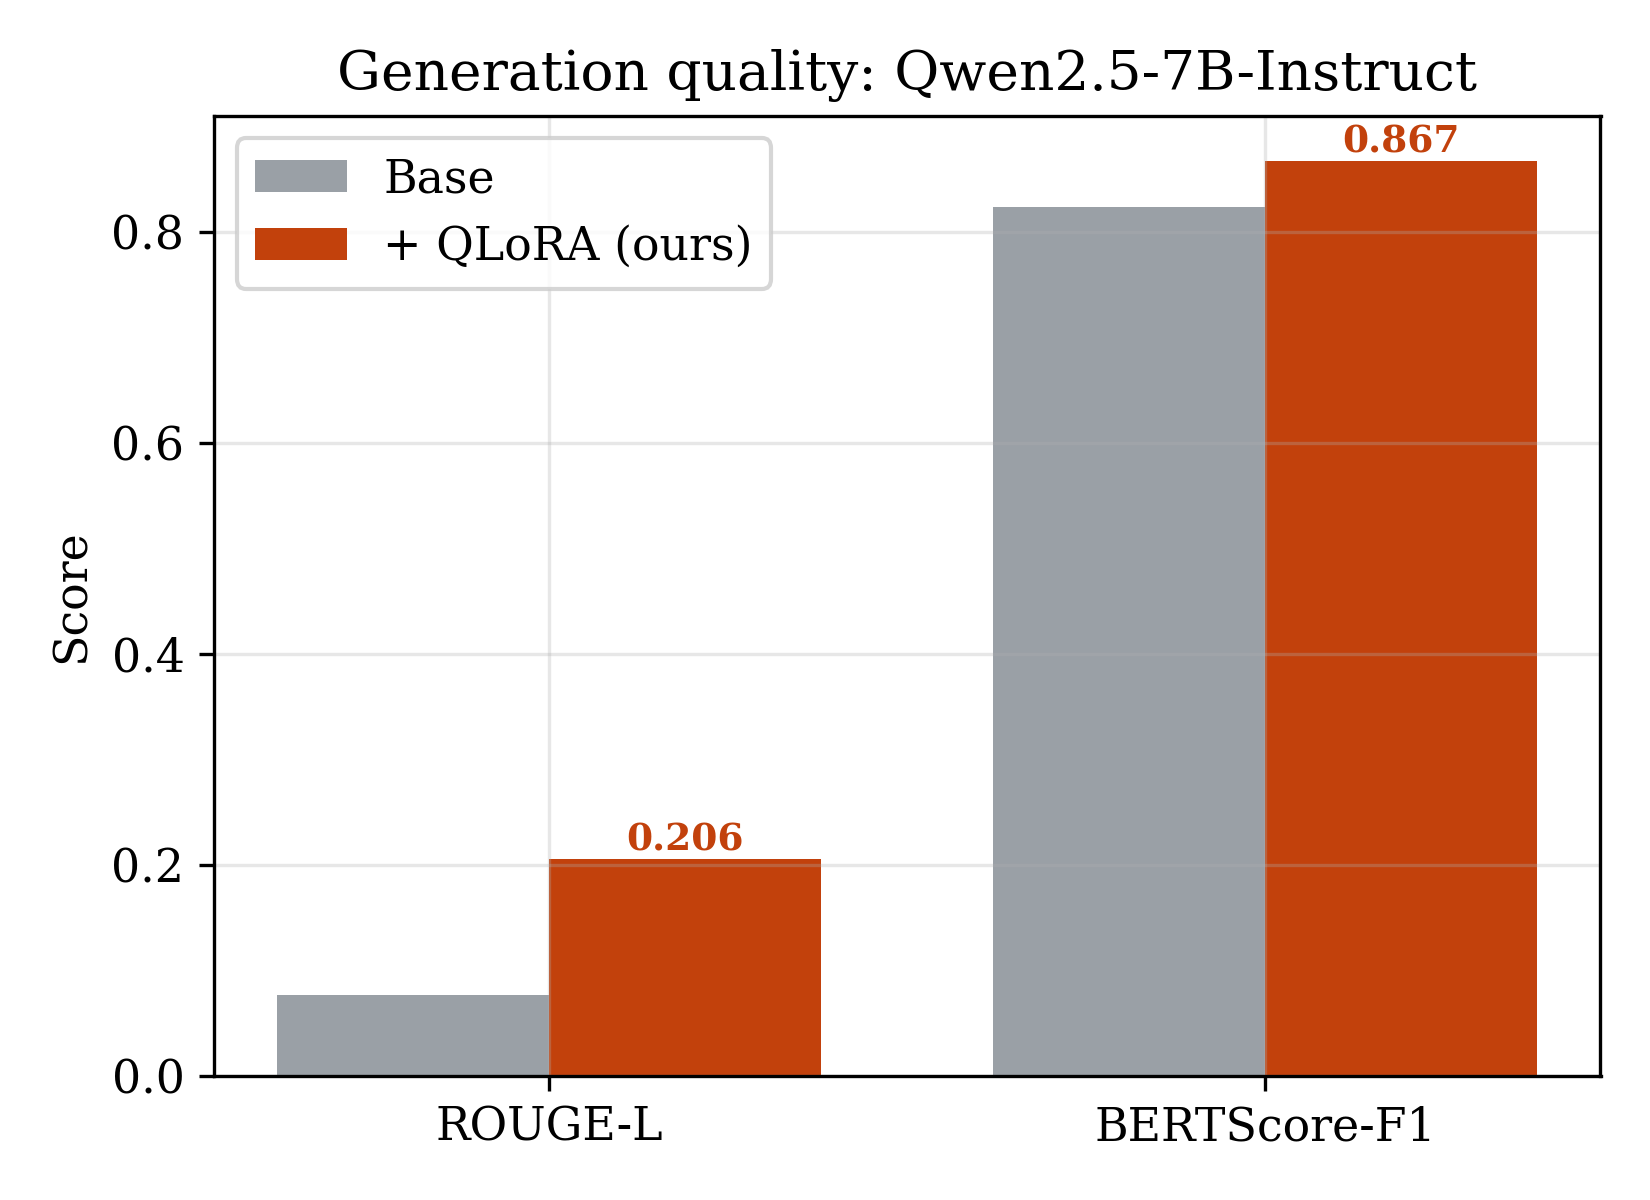
\includegraphics[width=0.85\columnwidth]{fig4_generation.png}
\caption{Generation quality: base Qwen versus our QLoRA-fine-tuned model.}
\label{fig:gen}
\end{figure}

\subsection{Comparison with the Base Paper}
Table~\ref{tab:vsbase} compares our system with the base paper~\cite{basepaper2026} on the same dataset.
We want to be careful here: this is \emph{not} a same-metric head-to-head, because the base paper only
reported an LLM-judge score on answers (about 49\% of answers scored $\geq 8/10$ with reranking, using
GPT-4.1), whereas we report retrieval metrics and reference-based generation metrics, and we use a small
local generator instead of a paid LLM. So the table compares the \emph{approach} and \emph{what each
system reports}, rather than claiming we beat their exact number. Our contribution is that we get large
relative gains from fine-tuning, on a free and fully local stack, and we measure the retrieval step that
they left unmeasured.

\begin{table}[t]
\caption{Approach comparison: base paper~\cite{basepaper2026} vs.\ FinRAG (ours).}
\label{tab:vsbase}
\centering
\small
\renewcommand{\arraystretch}{1.2}
\begin{tabular}{p{2.4cm}p{2.4cm}p{2.4cm}}
\toprule
Aspect & Cheng \textit{et al.} (base) & FinRAG (ours) \\
\midrule
Dataset & FinDER 10-Ks & FinDER 10-Ks \\
Embedding model & OpenAI, off-the-shelf & BGE, \textbf{fine-tuned} \\
Reranker & Jina v2, off-the-shelf & BGE, \textbf{fine-tuned} \\
Generator & GPT-4.1 (paid) & Qwen2.5-7B + QLoRA (local) \\
Query rewriting & GPT-4.1 & none \\
Retrieval metrics & not reported & \textbf{MRR/NDCG/Recall} \\
Answer evaluation & LLM judge ($\approx$49\% $\geq$8) & ROUGE/BLEU/BERTScore \\
Infrastructure & paid cloud APIs & single 12\,GB GPU, free \\
\bottomrule
\end{tabular}
\end{table}

\subsection{Qualitative Examples}
Table~\ref{tab:qual} shows two held-out examples (answers shortened). The base model often refuses or
stays vague, while the QLoRA model attempts a structured, on-style answer grounded in the retrieved text.
These are genuinely hard multi-step questions, so neither model is perfect, but the difference in style
and effort is visible.

\begin{table}[t]
\caption{Qualitative examples (shortened). Held-out questions.}
\label{tab:qual}
\centering
\small
\begin{tabular}{p{0.96\columnwidth}}
\toprule
\textbf{Q:} Howmet Aerospace Lehman settlement impact on Other expense, net \& liabilities? \\
\textit{Base:} ``No impact mentioned in the context provided.'' \\
\textit{Ours (QLoRA):} ``The reference discloses that the Lehman litigation was settled\,\ldots\ it does not give the exact amount, so the impact on future expenses or liabilities cannot be fully quantified.'' \\
\midrule
\textbf{Q:} Timing of revenue recognition for control transfer at Howmet Aerospace? \\
\textit{Ours (QLoRA):} ``Revenue is recognized when control transfers to the customer, typically at shipment or delivery when title and risk of loss pass\,\ldots\ advance payments are recorded as deferred revenue.'' \\
\bottomrule
\end{tabular}
\end{table}

\section{Discussion}
\label{sec:disc}
The clearest result is that \textbf{fine-tuning the retriever is the dominant lever}. A small embedding
model, once adapted to financial language and FinDER's terse query style, roughly tripled MRR@10. This
makes sense: the base model never saw such abbreviated queries, while fine-tuning teaches it the domain
vocabulary.

The more surprising result is that reranking and BM25 fusion stopped helping once the embedder was
fine-tuned. We think this happens because a strong domain retriever already returns a top list that is
almost entirely on-topic, so there is little for a reranker to fix, and a generic reranker can only
shuffle good results into a slightly worse order. This is different from the base paper, which found
reranking helpful on top of \emph{generic} embeddings. So our work does not contradict theirs --- it shows
that their conclusion depends on the retriever being generic.

We also learned a practical lesson about the reranker. Our first attempt trained it on negatives mined by
the \emph{base} model, and it passed a simple ``positive vs.\ easy negative'' check but then ranked very
badly in practice (MRR@10 collapsed to 0.03). The reason is that at inference the reranker sees hard,
look-alike candidates from the fine-tuned retriever, which it was never trained on. Re-mining the
negatives from the fine-tuned retriever fixed the collapse, although the reranker still did not beat
``no reranking'' at the top ranks. This matches the literature's advice that rerankers should be trained
on retriever-consistent hard negatives.

\section{Limitations}
FinDER is a hard benchmark, so the absolute scores are modest; our contribution is the relative
improvement from fine-tuning. Our evidence alignment uses TF--IDF and marks a single gold chunk per
question, which is conservative and adds some label noise. We do not use query rewriting or an LLM judge,
so our generation numbers cannot be compared directly to the base paper's answer score, which used a paid
LLM in a different configuration. Finally, the generator is a 7B model; a larger model would likely give
better raw answers, but our goal was a free, local system, not the highest possible answer quality.

\section{Conclusion and Future Work}
We presented FinRAG, a financial RAG system that fine-tunes its embedder, reranker, and generator on the
FinDER benchmark using only a single 12~GB consumer GPU and no paid services. Fine-tuning the embedder
improved retrieval MRR@10 by about $3\times$, and QLoRA improved generation quality, while our ablation
showed that retriever fine-tuning --- not reranking --- is the main driver in domain-specific RAG. In
future work we would like to try query rewriting with a small local model, multi-chunk gold labels for a
less conservative evaluation, and a larger generator to push answer quality further. All code, trained
configurations, and results are publicly available.\footnote{\url{https://github.com/Haroon-M-Bilal/finrag-}}

\begin{thebibliography}{00}
\bibitem{lewis2020rag} P. Lewis \textit{et al.}, ``Retrieval-augmented generation for knowledge-intensive NLP tasks,'' in \textit{Proc. NeurIPS}, 2020.
\bibitem{karpukhin2020dpr} V. Karpukhin \textit{et al.}, ``Dense passage retrieval for open-domain question answering,'' in \textit{Proc. EMNLP}, 2020.
\bibitem{robertson2009bm25} S. Robertson and H. Zaragoza, ``The probabilistic relevance framework: BM25 and beyond,'' \textit{Found. Trends Inf. Retr.}, vol. 3, no. 4, 2009.
\bibitem{khattab2020colbert} O. Khattab and M. Zaharia, ``ColBERT: Efficient and effective passage search via contextualized late interaction over BERT,'' in \textit{Proc. SIGIR}, 2020.
\bibitem{reimers2019sbert} N. Reimers and I. Gurevych, ``Sentence-BERT: Sentence embeddings using Siamese BERT-networks,'' in \textit{Proc. EMNLP}, 2019.
\bibitem{izacard2022contriever} G. Izacard \textit{et al.}, ``Unsupervised dense information retrieval with contrastive learning,'' \textit{TMLR}, 2022.
\bibitem{wang2022e5} L. Wang \textit{et al.}, ``Text embeddings by weakly-supervised contrastive pre-training,'' \textit{arXiv:2212.03533}, 2022.
\bibitem{ni2022gtr} J. Ni \textit{et al.}, ``Large dual encoders are generalizable retrievers,'' in \textit{Proc. EMNLP}, 2022.
\bibitem{xiao2023bge} S. Xiao \textit{et al.}, ``C-Pack: Packed resources for general Chinese embeddings,'' \textit{arXiv:2309.07597}, 2023.
\bibitem{thakur2021beir} N. Thakur \textit{et al.}, ``BEIR: A heterogeneous benchmark for zero-shot evaluation of information retrieval models,'' in \textit{Proc. NeurIPS Datasets}, 2021.
\bibitem{nogueira2019passage} R. Nogueira and K. Cho, ``Passage re-ranking with BERT,'' \textit{arXiv:1901.04085}, 2019.
\bibitem{cormack2009rrf} G. V. Cormack, C. L. A. Clarke, and S. B\"uttcher, ``Reciprocal rank fusion outperforms Condorcet and individual rank learning methods,'' in \textit{Proc. SIGIR}, 2009.
\bibitem{gao2022hyde} L. Gao \textit{et al.}, ``Precise zero-shot dense retrieval without relevance labels,'' \textit{arXiv:2212.10496}, 2022.
\bibitem{izacard2021fid} G. Izacard and E. Grave, ``Leveraging passage retrieval with generative models for open domain question answering,'' in \textit{Proc. EACL}, 2021.
\bibitem{asai2023selfrag} A. Asai \textit{et al.}, ``Self-RAG: Learning to retrieve, generate, and critique through self-reflection,'' \textit{arXiv:2310.11511}, 2023.
\bibitem{vaswani2017attention} A. Vaswani \textit{et al.}, ``Attention is all you need,'' in \textit{Proc. NeurIPS}, 2017.
\bibitem{hu2021lora} E. J. Hu \textit{et al.}, ``LoRA: Low-rank adaptation of large language models,'' \textit{arXiv:2106.09685}, 2021.
\bibitem{dettmers2023qlora} T. Dettmers \textit{et al.}, ``QLoRA: Efficient finetuning of quantized LLMs,'' in \textit{Proc. NeurIPS}, 2023.
\bibitem{qwen2024} Qwen Team, ``Qwen2.5 technical report,'' \textit{arXiv:2412.15115}, 2024.
\bibitem{touvron2023llama} H. Touvron \textit{et al.}, ``Llama 2: Open foundation and fine-tuned chat models,'' \textit{arXiv:2307.09288}, 2023.
\bibitem{jiang2023mistral} A. Q. Jiang \textit{et al.}, ``Mistral 7B,'' \textit{arXiv:2310.06825}, 2023.
\bibitem{araci2019finbert} D. Araci, ``FinBERT: Financial sentiment analysis with pre-trained language models,'' \textit{arXiv:1908.10063}, 2019.
\bibitem{wu2023bloomberggpt} S. Wu \textit{et al.}, ``BloombergGPT: A large language model for finance,'' \textit{arXiv:2303.17564}, 2023.
\bibitem{chen2021finqa} Z. Chen \textit{et al.}, ``FinQA: A dataset of numerical reasoning over financial data,'' in \textit{Proc. EMNLP}, 2021.
\bibitem{finder2025} Linq AI Research, ``FinDER: Financial dataset for question answering and evaluating retrieval-augmented generation,'' \textit{arXiv:2504.15800}, 2025.
\bibitem{es2023ragas} S. Es \textit{et al.}, ``RAGAS: Automated evaluation of retrieval augmented generation,'' \textit{arXiv:2309.15217}, 2023.
\bibitem{lin2004rouge} C.-Y. Lin, ``ROUGE: A package for automatic evaluation of summaries,'' in \textit{Proc. ACL Workshop}, 2004.
\bibitem{papineni2002bleu} K. Papineni \textit{et al.}, ``BLEU: A method for automatic evaluation of machine translation,'' in \textit{Proc. ACL}, 2002.
\bibitem{zhang2020bertscore} T. Zhang \textit{et al.}, ``BERTScore: Evaluating text generation with BERT,'' in \textit{Proc. ICLR}, 2020.
\bibitem{johnson2019faiss} J. Johnson, M. Douze, and H. J\'egou, ``Billion-scale similarity search with GPUs,'' \textit{IEEE Trans. Big Data}, 2019.
\bibitem{manning2008ir} C. D. Manning, P. Raghavan, and H. Sch\"utze, \textit{Introduction to Information Retrieval}. Cambridge Univ. Press, 2008.
\bibitem{basepaper2026} Y. Cheng \textit{et al.}, ``Enhancing financial report question-answering: A retrieval-augmented generation system with reranking analysis,'' \textit{arXiv:2603.16877}, 2026.
\end{thebibliography}

\end{document}
